%\addtocounter{chapter}{-1}
\chapter{Advice for the reader}

\section{Prerequisites}
As explained in the preface,
the main prerequisite is some amount of mathematical maturity.
This means I expect the reader to know how
to read and write a proof, follow logical arguments, and so on.

I also assume the reader is familiar with basic terminology
about sets and functions (e.g.\ ``what is a bijection?'').
If not, one should consult \Cref{ch:sets_functions}.

\section{Deciding what to read}
There is no need to read this book in linear order:
it covers all sorts of areas in mathematics,
and there are many paths you can take.
In \Cref{ch:sales}, I give a short overview for each part
explaining what you might expect to see in that part.

For now, here is a brief chart showing
how the chapters depend on each other;
again see \Cref{ch:sales} for details.
Dependencies are indicated by arrows;
dotted lines are optional dependencies.
\textbf{I suggest that you simply pick a chapter you find interesting,
and then find the shortest path.}
With that in mind, I hope the length of the entire PDF is not intimidating.

%\chapter*{Graph of Chapter Dependencies}
%\addcontentsline{toc}{chapter}{Graph of Chapter Dependencies}

\bgroup
\renewcommand{\href}[1]{} % temp disable links
\renewcommand{\solidwidth}{0.7pt}
\renewcommand{\boldwidth}{1.5pt}

\setcounter{diagheight}{50}
\begin{chart}
\reqhalfcourse 20,45:{Ch 1,3-5}{Abs Alg}{}
\reqhalfcourse 55,45:{Ch 2,6-8}{Topology}{}
\halfcourse 33,45:{Ch 9-15,18}{Lin Alg}{}
\halfcourse 5,35:{Ch 16}{Grp Act}{}
\halfcourse 5,24:{Ch 17}{Grp Classif}{}
\halfcourse 30,35:{Ch 19-22}{Rep Th}{}
\halfcourse 45,43:{Ch 23-25}{Quantum}{}
\halfcourse 64,38:{Ch 26-30}{Calc}{}
\halfcourse 64,30:{Ch 31-33}{Cmplx Ana}{}
\halfcourse 55,20:{Ch 34-41}{Measure/Pr}{}
\halfcourse 48,28:{Ch 42-45}{Diff Geo}{}
\halfcourse 40,10:{Ch 46-51}{Alg NT 1}{}
\halfcourse 40,0:{Ch 52-56}{Alg NT 2}{}
\halfcourse 23,10:{Ch 57-59}{Alg Top 1}{}
\halfcourse 20,28:{Ch 60-63}{Cat Th}{}
\halfcourse 23,0:{Ch 64-69}{Alg Top 2}{}
\halfcourse 6,10:{Ch 70-74}{Alg Geo 1}{}
\halfcourse 6,0:{Ch 75-80}{Alg Geo 2-3}{}
\reqhalfcourse 5,45:{Ch 81-87}{Set Theory}{}

%% Basic alg ch
\prereqc 20,45,30,35;0:    % Abs Alg -> Rep Th
\coreqc  20,45,33,45;0:    % Abs Alg -> Lin Alg
\prereqc 33,45,30,35;0:    % Lin Alg -> Rep Th
\prereqc 33,45,45,43;0:    % Lin Alg -> Quantum
%% Category theory
\prereqc 20,45,20,28;0:    % Grp -> Cat Th
\coreqc  20,45,20,28;0:    % Abs Alg -> Cat Th
\coreqc  33,45,20,28;80:   % Lin Alg -> Cat Th
\coreqc  55,45,20,28;-40:  % Top -> Cat Th
\coreqc  20,28,30,35;0:    % Cat Th -> Rep Th
%% Group theory chain
\prereqc 20,45,5,35;0:     % Grp -> Grp Act
\prereqc  5,35,5,24;0:     % Grp Act -> Grp Class
%% Analysis chain
\prereqc 33,45,48,28;30:   % Lin Alg -> Diff Geo
\prereqc 55,45,64,38;0:    % Top -> Diff Geo
\coreqc  64,38,48,28;50:   % Calc -> Diff Geo
\prereqc 55,45,48,28;10:   % Top -> Diff Geo
\prereqc 55,45,64,38;0:    % Top -> Calc
\coreqc  64,38,64,30;0:    % Calc -> Cmplx Ana
\prereqc 55,45,64,30;-10:  % Top -> Cmplx Ana
\prereqc 55,45,55,20;0:    % Top -> Meas/Pr
\coreqc  64,38,55,20;50:   % Calc -> Meas/Pr
%% Alg Geom
\prereqc 6,10,6,0;0:       % AG1 -> AG2
\prereqc 20,45,6,10;0:     % Abs Alg -> AG1
\prereqc 55,45,6,10;-40:   % Top -> AG1
\coreqc  20,28,6,10;0:     % Cat Th -> AG1
\prereqc 20,28,6,0;-18:    % Cat -> AG2
%% Alg Top
\prereqc 23,10,23,0;0:     % AT1 -> AT2
\prereqc 55,45,23,10;0:    % Top -> AT1
\prereqc  5,35,23,10;20:   % Grp Act -> AT1
\coreqc 23,10,20,28;20:    % AT1 -> Cat
\prereqc 20,28,23,0;-190:  % Cat -> AT2
%% Alg NT
\prereqc 40,10,40,0;0:     % ANT1 -> ANT2
\prereqc 20,45,40,10;-40:  % Abs Alg -> ANT1
\prereqc 33,45,40,10;50:   % Lin Alg -> ANT1
\prereqc  5,35,40,0;10:    % Grp Act -> ANT2
\end{chart}
\egroup

\newpage

\section{Questions, exercises, and problems}
In this book, there are three hierarchies:
\begin{itemize}
	\ii An inline \vocab{question} is intended to be offensively easy,
	mostly a chance to help you internalize definitions.
	If you find yourself unable to answer one or two of them,
	it probably means I explained it badly and you should complain to me.
	But if you can't answer many,
	you likely missed something important: read back.
	\ii An inline \vocab{exercise} is more meaty than a question,
	but shouldn't have any ``tricky'' steps.
	Often I leave proofs of theorems and propositions as exercises
	if they are instructive and at least somewhat interesting.
	\ii Each chapter features several trickier \vocab{problems} at the end.
	Some are reasonable, but others are legitimately
	difficult olympiad-style problems.
	\gim Harder problems are marked with up to
	three chili peppers (\scalebox{0.7}{\chili}), like this paragraph.

	In addition to difficulty annotations,
	the problems are also marked by how important they are to the big picture.
	\begin{itemize}
		\ii \textbf{Normal problems},
		which are hopefully fun but non-central.
		\ii \textbf{Daggered problems},
		which are (usually interesting) results that one should know,
		but won't be used directly later.
		\ii \textbf{Starred problems},
		which are results which will be used later
		on in the book.\footnote{This is to avoid the classic
			``we are done by PSet 4, Problem 8''
			that happens in college sometimes,
			as if I remembered what that was.}
	\end{itemize}
\end{itemize}
Several hints and solutions can be found in \Cref{app:hints,app:sol}.

\begin{center}
	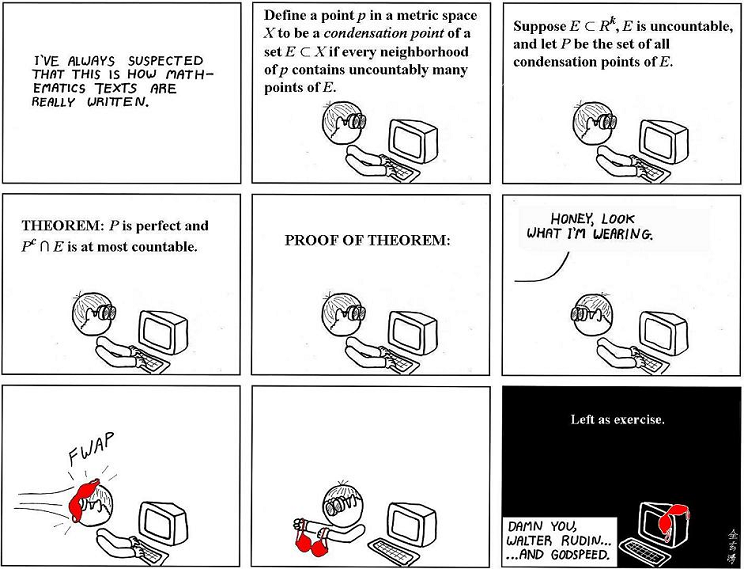
\includegraphics[width=14cm]{media/abstruse-goose-exercise.png}
	\\ \scriptsize Image from \cite{img:exercise}
\end{center}

% I personally find most exercises to not be that interesting, and I've tried to keep boring ones to a minimum.
% Regardless, I've tried hard to pick problems that are fun to think about and, when possible, to give them
% the kind of flavor you might find on the IMO or Putnam (even when the underlying background is different).

\section{Paper}
At the risk of being blunt,
\begin{moral}
Read this book with pencil and paper.
\end{moral}
Here's why:

\begin{center}
	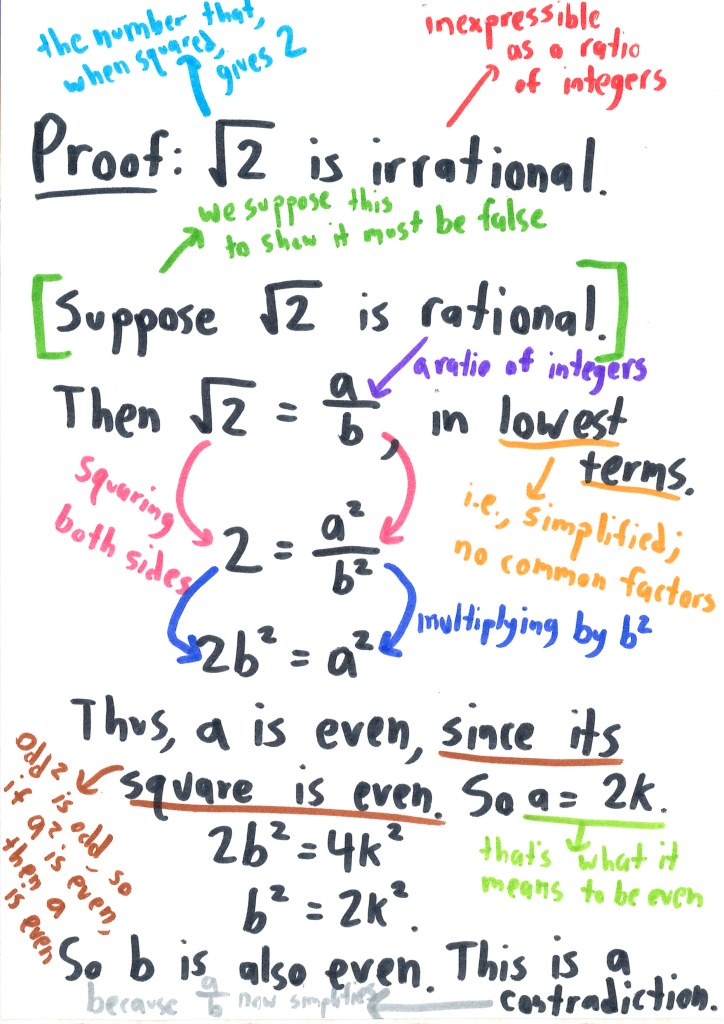
\includegraphics[width=0.5\textwidth]{media/read-with-pencil.jpg}
	\\ \scriptsize Image from \cite{img:read_with_pencil}
\end{center}
You are not God.
You cannot keep everything in your head.\footnote{
	See also \url{https://usamo.wordpress.com/2015/03/14/writing/}
	and the source above.}
If you've printed out a hard copy, then write in the margins.
If you're trying to save paper,
grab a notebook or something along with the ride.
Somehow, some way, make sure you can write. Thanks.

\section{On the importance of examples}
I am pathologically obsessed with examples.
In this book, I place all examples in large boxes to draw emphasis to them,
which leads to some pages of the book simply consisting of sequences of boxes
one after another. I hope the reader doesn't mind.

I also often highlight a ``prototypical example'' for some sections,
and reserve the color red for such a note.
The philosophy is that any time the reader sees a definition
or a theorem about such an object, they should test it
against the prototypical example.
If the example is a good prototype, it should be immediately clear
why this definition is intuitive, or why the theorem should be true,
or why the theorem is interesting, et cetera.

Let me tell you a secret.  Whenever I wrote a definition or a theorem in this book,
I would have to recall the exact statement from my (quite poor) memory.
So instead I often consider the prototypical example,
and then only after that do I remember what the definition or the theorem is.
Incidentally, this is also how I learned all the definitions in the first place.
I hope you'll find it useful as well.

\section{Conventions and notations}
This part describes some of the less familiar notations and definitions
and settles for once and for all some annoying issues
(``is zero a natural number?'').
Most of these are ``remarks for experts'':
if something doesn't make sense,
you probably don't have to worry about it for now.

A full glossary of notation used can be found in the appendix.

\subsection{Natural numbers are positive}
The set $\NN$ is the set of \emph{positive} integers, not including $0$.
In the set theory chapters, we use $\omega = \{0, 1, \dots\}$
instead, for consistency with the rest of the book.

\subsection{Sets and equivalence relations}
This is brief, intended as a reminder for experts.
Consult \Cref{ch:sets_functions} for full details.

An \vocab{equivalence relation} on a set $X$ is a relation $\sim$
which is symmetric, reflexive, and transitive.
An equivalence relation partitions $X$
into several \vocab{equivalence classes}.
We will denote this by $X / {\sim}$.
An element of such an equivalence class is a
\vocab{representative} of that equivalence class.

I always use $\cong$ for an ``isomorphism''-style relation
(formally: a relation which is an isomorphism in a reasonable category).
The only time $\simeq$ is used in the Napkin is for homotopic paths.

I generally use $\subseteq$ and $\subsetneq$ since these are non-ambiguous,
unlike $\subset$.  I only use $\subset$ on rare occasions in which equality
obviously does not hold yet pointing it out would be distracting.
For example, I write $\QQ \subset \RR$
since ``$\QQ \subsetneq \RR$'' is distracting.

I prefer $S \setminus T$ to $S - T$.

The power set of $S$ (i.e.,\ the set of subsets of $S$),
is denoted either by $2^S$ or $\mathcal P(S)$.

\subsection{Functions}
This is brief, intended as a reminder for experts.
Consult \Cref{ch:sets_functions} for full details.

Let $X \taking f Y$ be a function:
\begin{itemize}
\ii By $f\pre(T)$ I mean the \vocab{pre-image}
\[ f\pre(T) \defeq \left\{ x \in X \mid f(x) \in T \right\}.  \]
This is in contrast to the $f\inv(T)$ used in the rest of the world;
I only use $f\inv$ for an inverse \emph{function}.

By abuse of notation, we may abbreviate $f\pre(\{y\})$ to $f\pre(y)$.
We call $f\pre(y)$ a \vocab{fiber}.

\ii By $f\im(S)$ I mean the \vocab{image}
\[ f\im(S) \defeq \left\{ f(x) \mid x \in S \right\}. \]
Almost everyone else in the world uses $f(S)$
(though $f[S]$ sees some use, and $f``(S)$ is often used in logic)
but this is abuse of notation,
and I prefer $f\im(S)$ for emphasis.
This image notation is \emph{not} standard.

\ii If $S \subseteq X$, then the \vocab{restriction} of $f$ to $S$
is denoted $f \restrict{S}$,
i.e.\ it is the function $f \restrict{S} \colon S \to Y$.

\ii Sometimes functions $f \colon X \to Y$
are \emph{injective} or \emph{surjective};
I may emphasize this sometimes by writing
$f \colon X \injto Y$ or $f \colon X \surjto Y$, respectively.
\end{itemize}

\subsection{Cycle notation for permutations}
\label{subsec:cycle_notation}

Additionally, a permutation on a finite set may be denoted
in \emph{cycle notation},
as described in say \url{https://en.wikipedia.org/wiki/Permutation#Cycle_notation}.
For example the notation $(1 \; 2 \; 3 \; 4)(5 \; 6 \; 7)$
refers to the permutation with
$1 \mapsto 2$, $2 \mapsto 3$, $3 \mapsto 4$, $4 \mapsto 1$,
$5 \mapsto 6$, $6 \mapsto 7$, $7 \mapsto 5$.
Usage of this notation will usually be obvious from context.

\subsection{Rings}
All rings have a multiplicative identity $1$ unless otherwise specified.
We allow $0=1$ in general rings but not in integral domains.

\textbf{All rings are commutative unless otherwise specified.}
There is an elaborate scheme for naming rings which are not commutative,
used only in the chapter on cohomology rings:

\begin{center}
	\small
	\begin{tabular}[h]{|c|cc|}
		\hline
		& Graded & Not Graded \\ \hline
		$1$ not required & graded pseudo-ring & pseudo-ring \\
		Anticommutative, $1$ not required & anticommutative pseudo-ring & N/A \\
		Has $1$ & graded ring & N/A \\
		Anticommutative with $1$ & anticommutative ring & N/A \\ 
		Commutative with $1$ & commutative graded ring & ring \\ \hline
	\end{tabular}
\end{center}

On the other hand, an \emph{algebra} always has $1$,
but it need not be commutative.

\subsection{Choice}
We accept the Axiom of Choice, and use it freely.

\section{Further reading}
The appendix \Cref{ch:refs} contains a list of resources I like,
and explanations of pedagogical choices that I made for each chapter.
I encourage you to check it out.

In particular, this is where you should go for further reading!
There are some topics that should be covered in the Napkin,
but are not, due to my own ignorance or laziness.
The references provided in this appendix should hopefully help partially
atone for my omissions.
